\documentclass[a4paper]{report}
%\usepackage[colorlinks=true, linkcolor=black]{bookmark} 
\usepackage{bookmark} 
\usepackage[italian]{babel}
\usepackage[latin1]{inputenc}
\usepackage[T1]{fontenc}
\usepackage{indentfirst}
\usepackage{booktabs}
\usepackage{amsmath,amssymb}
\usepackage{graphicx}
\graphicspath{{Immagini/}}
\usepackage{listings}
\lstset{language=C,
		gobble=16,
		breaklines=true}
\usepackage{caption}
\captionsetup[table]{position=top}
\usepackage{float}
\author{E. Anfuso \and A. Caligiuri}
\title{Full Adder TSPC}
\date{}
\begin{document}
	\maketitle
	\tableofcontents
	\chapter{Introduzione}
	\section{Obiettivi del progetto}
	
	\section{Requisiti e prestazioni attese}

	\begin{itemize}
		\item a
		\item b
	\end{itemize}
	
	\chapter{Preparazione dispositivo}
	\section{Funzionalit� previste}
	
		\section{Il microcontrollore}

		\section{Le funzioni in C}	
		\subsection{\textit{findMax}}
				
		\begin{lstlisting}
		int findMax (float array [], int size);
		int findMax (float array [], int size){
			int index=0;
			float max=array[0];
			for (int i=1; i<size; i++){
				if (array[i]>max){
				max=array[i];
				index=i;
				}
			}
			return index;
		} 
		\end{lstlisting}
		
		\begin{table}[htb]
			\caption{Dimensionamento filtro RC per generazione segnale di misura}
			\label{tab:filtroRC}
			\centering
			\begin{tabular}{c*{3}{c}}
				\toprule
				Frequenza sinusoide (Hz) & R ($\Omega$)& C(F) & $ f_{t} $(Hz)\\
				\midrule
				100 & 100k & 10n & 159\\
				\bottomrule
			\end{tabular}
		\end{table}
		
	\begin{figure}[H]
		\centering%
		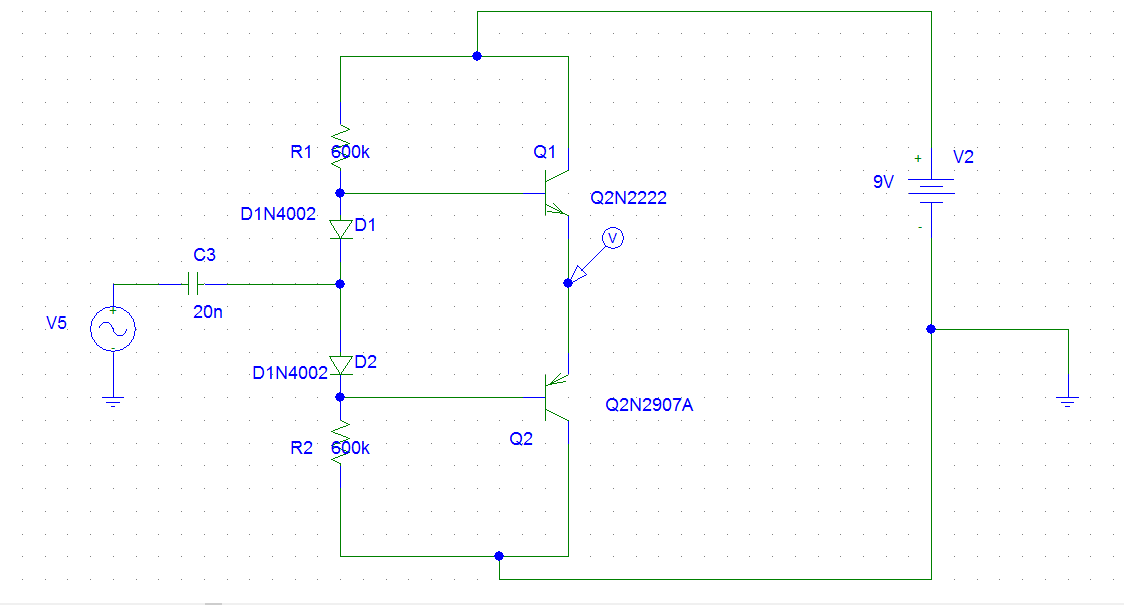
\includegraphics[width=0.8\textwidth]{ClasseAB.png}%
		\caption{Circuito classe AB\label{fig:ClasseAB}}%
	\end{figure}
	
	%\section{Misurazioni}
	%\section{Ottimizzazioni}
	\bookmarksetup{startatroot}
	\chapter{Conclusioni e sviluppi potenziali}
	%\chapter{Riferimenti}
	\chapter{Allegati}
	Si allega alla seguente relazione:
	\begin{itemize}
		\item 
	\end{itemize}
	
	\cleardoublepage
	\addcontentsline{toc}{chapter}{\bibname}
	\begin{thebibliography}{9}
		\bibitem{pwm}
		Michael Lemmon (2009-02-01),
		�What is the RC circuit's response to a PWM signal?�,
		\url{http://www3.nd.edu/~lemmon/courses/ee224/web-manual/web-manual/lab8a/node5.html}.
	\end{thebibliography}
\end{document}


